%&program=pdflatex

\documentclass[12pt]{article}
\usepackage{geometry} % see geometry.pdf on how to lay out the page. There's lots.
\usepackage{graphics} 
\geometry{a4paper} % or letter or a5paper or ... etc
% \geometry{landscape} % rotated page geometry


% See the ``Article customise'' template for come common customisations

\title{
   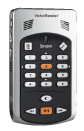
\includegraphics{vrstream.jpg} \\
   iStream User Guide}
\author{Gregory Kearney}


%%% BEGIN DOCUMENT
\begin{document}




\maketitle
\tableofcontents

\section{Introduction}
iStream is a Macintosh utility to manage a VictorReader Stream digital talking book player manufactured by Humanware. iStream simplifies the copying of Daisy digital talking books and other media to the VictorReader Stream player as well as permitting the user to convert and install a wide range of audio formats from Apple's iTunes application as well as from the file system itself.

iStream can also create the VictorReader Stream's special bookmarked folder, backup the Stream and delete files from the VictorReader Stream as needed.

\section{Connecting the VictorReader Stream to your Macintosh}
You will connect the VictorReader Stream to your Macintosh by means of the USB cable that come with the VictorReader Stream. The VictorReader Stream will appear to the Macintosh as an external USB mass storage device. You can copy file to and from with the Finder as well as with iStream.

\section{iStream Commands}
The iStream application has two types of commands. Menu command which install various media types and on screen button commands with perform various maintenance tasks such as creating directories, backup tasks and removal of media.
\subsection{Menu Commands}
\subsubsection{File Menu Commands}
\begin{description}
\item[ Install iTunes... (Command-I)] This command is used to install selected tracks from iTunes onto the VictorReader Stream. To use this command first go to iTunes and select any unprotected tracks you wish to import. Then return to iStream and choose this command. iStream will ask for the directory you wish to install the selected tracks to. iStream will convert any tracks that are in a format that VictorReader Stream can not play to MP3 format and install the tracks in the selected directory on the reader.
\item[ Install Daisy... (Command-D)] This command is used to install Daisy digital talking books to the VictorReader Stream it will ask you to locate the directory holding the books files and the location where you want the book installed. It will then create a new directory on the VictorReader Stream using the books title and copy all the required files to that new directory.
\item[ Install Text... (Command-T)] This command is used to install Text and HTML files to the VictorReader Stream it will ask you to locate the text file and the location where you want the file installed. iStream will copy the file to the selected location on the VictorReader Stream.
\item[ Install Audio... (Command-A)] This command is used to install audio files to the VictorReader Stream that are not installed in iTunes. It will ask you to locate the audio file and the location where you want the file installed. iStream will convert the file to MP3 if it is in a format that VictorReader Stream does not support and copy the file to the selected location on the VictorReader Stream.
\item[ Backup (Command-B)] This command is used to backup the contents VictorReader Stream. It will ask for the root directory or any sub directory of your VictorReader Stream and write a non-distructive backup of that directory to a directory named VRBackup in your home directory.
\item[ Create Folders (Command-B)] This command is used to create the various special bookmarked directories on the VictorReader Stream if they do not already exist. It will also create a directory named VRBackup in your home directory.
\end{description}
\subsection{Button Commands}
The button command are on the iStream main window which also has a busy/not busy indicator.
\begin{description}
\item[ Create Folders (Command-B)] This command is used to create the various special bookmarked directories on the VictorReader Stream if they do not already exist. It will also create a directory named VRBackup in your home directory.
\item[ Backup (Command-B)] This command is used to backup the contents VictorReader Stream. It will ask for the root directory or any sub directory of your VictorReader Stream and write a non-distructive backup of that directory to a directory named VRBackup in your home directory.
\item[ Remove] This command is used to remove contents VictorReader Stream. It will ask for the file or directory to remove and will place that file or directory into the trash on your computer. Unlike the other commands remove must be accessed via VoiceOver or with the mouse.
\end{description}
\section{Audio Conversion}
iStream will permit you to install audio files which are not supported by the VictorReader Stream. This is done by converting none MP3 and WAV files to MP3 files when you use iStream to install them. This is don on both the Install iTunes and Install Audio options.  If a file can not be converted, an iTunes protected file for example it is skipped. Below is a list of the various formats which can be converted.

\begin{itemize}
\item M4A (ACC unprotected)
\item M4B (ACC audiobook)
\item OGG
\item AVI
\item AU
\item MOV (QuickTime)
\item AIFF, AIF
\item 3GP
\item FLV (Flash)
\end{itemize}

Other formats can be added please contact the author at gkearney@gmail.com



\end{document}